% !TEX root = ../main.tex
% !TEX spellcheck = en_GB

\chapter{Test}
In this section an short introduction to how this project has used test from beginning to the end will be described.

\section{Module tests}
The goal of the module tests is to determine if the used modules are able to perform the actions demanded by the \nameref{chap:requirements}.

Module tests has been performed on the \SARA GSM module, \GPS GPS module, and the \SDsock µSD-card socket with µSD-card inserted.

\subsection{GSM \SARA}
The module test of the GSM \SARA tests if the module is able to send a simple string to a known server.

The used test command is
\begin{quote}
	AT+USOST=\textit{SOCK},"\textit{IP}",\textit{PORT},11,"Hello World"
\end{quote}
Where \textit{SOCK} is decided by the \SARA module, and \textit{IP} and \textit{PORT} are decided by the server.

\begin{table}[H]
	\centering
	\begin{tabularx}{\textwidth}{p{4.3cm} X X}
		\toprule
		\textbf{Action} & \textbf{Expected outcome} & \textbf{Outcome} \\
		\midrule
		Send test command, via a USB to UART module, to \MKR coded with an Arduino Sketch forwarding the input to the \SARA. & The server log shows "Hello World". & Success. For more information see transcript in appendix \cref{app:GSMcomm}. \\
		\bottomrule
	\end{tabularx}
	\caption{Module test of \SARA GSM module.}
	\label{AT:modGSM}
\end{table}

\subsection{GPS \GPS}
The GPS module is tested by connecting it to a USB to UART module and sending the appropriate UBX commands. The setting is outdoors as to achieve the most precise localization.

Before this, the below command CFG-PRT (Port Configuration for UART) \cite[p.~119-120]{NEO7_proto}, must be sent to the GPS module, to only enable UBX commands in and out, and set the baud rate to \num{9600}:

\noindent
\textit{0xB5620600140001000000D00800008025000001000100000000009A79}

\begin{table}[H]
	\centering
	\begin{tabularx}{\textwidth}{p{4.3cm} X X}
		\toprule
		\textbf{Action} & \textbf{Expected outcome} & \textbf{Outcome} \\
		\midrule
		Send \textit{0xB562010700000819} (UBX-NAV-PVT/Get location) from computer to GPS module via USB to UART with \num{9600} baud. & Receive \SI{92}{\byte} according to \cite[p.~160-161]{NEO7_proto}. & \SI{92}{\byte} received. Output shown in \cref{app:GPSmodtest}. \\
		\midrule
		Input coordinates achieved from above test into Google Maps. & Pin is placed at the location above command was issued at. & Pin is placed at the location the command was issued. \\
		\bottomrule
	\end{tabularx}
	\caption{Module test of \GPS GPS module.}
	\label{AT:modGPS}
\end{table}

\subsection{\SDsock socket and µSD-card}
Before the test, use \textit{dd} on a Linux device, to clear the µSD-card with \\
\mintinline{bash}{dd if=/dev/zero of=/dev/sdX}, where sdX is the µSD-card.

\begin{table}[H]
	\centering
	\begin{tabularx}{\textwidth}{p{4.3cm} X X}
		\toprule
		\textbf{Action} & \textbf{Expected outcome} & \textbf{Outcome} \\
		\midrule
		Use an Arduino Sketch driver for the \MKR to save the string "Hello World" to the µSD-card via SPI.
		Remove the µSD-card from the \SDsock socket and read it on a Linux device using \textit{dd} to a file. & The output file shows "Hello World". & \\
		\bottomrule
	\end{tabularx}
	\caption{Module test of \SDsock socket and µSD-card.}
	\label{AT:modSD}
\end{table}

\section{Integration tests}
The integration tests are much like the module tests, except for the \MKR being the facilitator of the data.

\subsection{\MKR with \SARA}
The used test command is
\begin{quote}
	AT+USOST=\textit{SOCK},"\textit{IP}",\textit{PORT},11
\end{quote}
Where \textit{SOCK} is decided by the \SARA module, and \textit{IP} and \textit{PORT} are decided by the server.

\begin{table}[H]
	\centering
	\begin{tabularx}{\textwidth}{p{4.3cm} X X}
		\toprule
		\textbf{Action} & \textbf{Expected outcome} & \textbf{Outcome} \\
		\midrule
		Send test command from \MKR to \SARA via UART. &
		\SARA responds with @. Debugger shows @ in buffer & Hex value for @ (0x40) shown in debugger.\\
		Send "Hello World" & The server log shows "Hello World". & The server log shows "Hello World".\\
		\bottomrule
	\end{tabularx}
	\caption{Integration test of \MKR and \SARA GSM module.}
	\label{AT:intGSM}
\end{table}

\subsection{\MKR with \GPS}
Before this, the command CFG-PRT (Port Configuration for UART) \cite[p.~119-120]{NEO7_proto}, must be sent to the GPS module.

\begin{table}[H]
	\centering
	\begin{tabularx}{\textwidth}{p{4.3cm} X X}
		\toprule
		\textbf{Action} & \textbf{Expected outcome} & \textbf{Outcome} \\
		\midrule
		Send \textit{0xB562010700000819} (UBX-NAV-PVT/Get location) from \MKR, with debugger on, to GPS module via UART with \num{9600} baud. & Receive \num{92} bytes according to \cite[p.~160-161]{NEO7_proto}. & \SI{92}{\byte} received. Output shown in \cref{app:GPSinttest}. \\
		Input coordinates achieved from above test into Google Maps. & Pin is placed at the location above command was issued at. & Pin is placed at the location the command was issued. \\
		\bottomrule
	\end{tabularx}
	\caption{Integration test of \MKR and \GPS GPS module.}
	\label{AT:intGPS}
\end{table}

\subsection{\MKR with \SDsock and µSD-card}
Before the test, use \textit{dd} on a Linux device, to clear the µSD-card with\\
\mintinline{bash}{dd if=/dev/zero of=/dev/sdX}, where sdX is the µSD-card.

\begin{table}[H]
	\centering
	\begin{tabularx}{\textwidth}{p{4.3cm} X X}
		\toprule
		\textbf{Action} & \textbf{Expected outcome} & \textbf{Outcome} \\
		\midrule
		Use the \MKR to save the string "Hello World" to the µSD-card via SPI.
		Remove the µSD-card from the \SDsock socket and read it on a Linux device using \textit{dd} to a file. & The output file shows "Hello World". & \\
		\bottomrule
	\end{tabularx}
	\caption{Integration test of \MKR and \SDsock socket and µSD-card.}
	\label{AT:intSD}
\end{table}

\section{Acceptance Tests}
The goal of the acceptance test is to test the system as a whole.
Due to time constraints, two acceptance tests are produced, one with and one without the \SDsock and µSD-card.

Acceptance tests are carried out outdoors to ensure good GPS signal quality.

\begin{table}[H]
	\centering
	\begin{tabularx}{\textwidth}{p{4.3cm} X X}
		\toprule
		\textbf{Action} & \textbf{Expected outcome} & \textbf{Outcome} \\
		\midrule
		Power on \systemName. Wait \SI{5}{\minute}. & One valid location data point is shown on the server. & \\
		Wait \SI{5}{\minute}. & The server still shows one valid data point. & \\
		Wait \SI{15}{\minute}. & The server shows \numrange{15}{20} valid location data points. & \\
		A GPS location from the server is put into Google Maps. & Google Maps shows the location where the \systemName was turned on. & \\
		\bottomrule
	\end{tabularx}
	\caption{Acceptance test of \systemName with  \SDsock socket and µSD-card.}
	\label{AT:withSD}
\end{table}

\begin{table}[H]
	\centering
	\begin{tabularx}{\textwidth}{p{4.3cm} X X}
		\toprule
		\textbf{Action} & \textbf{Expected outcome} & \textbf{Outcome} \\
		\midrule
		Power on \systemName. Wait \SI{5}{\minute}. & \numrange{1}{5} valid data points are shown on the server. & The server receives $\approx$ 5 valid values pr. minute, but stops receiving after \SI{2}{\minute}, due to an unknown interrupt error on the \SAMD. Output shown in \cref{fig:accepttestconsole}. \\
		Wait \SI{5}{\minute}. & \numrange{5}{10} valid data points are shown on the server. & \\
		Wait \SI{15}{\minute}. & The server shows \numrange{15}{25} valid location data points. & \\
		A GPS location from the server is put into Google Maps. & Google Maps shows the location where the \systemName was turned on. & The location is correct. See \cref{fig:accepttestmaps}. \\
		\bottomrule
	\end{tabularx}
	\caption{Acceptance test of \systemName without \SDsock socket and µSD-card.}
	\label{AT:withoutSD}
\end{table}

\begin{figure}
	\centering
	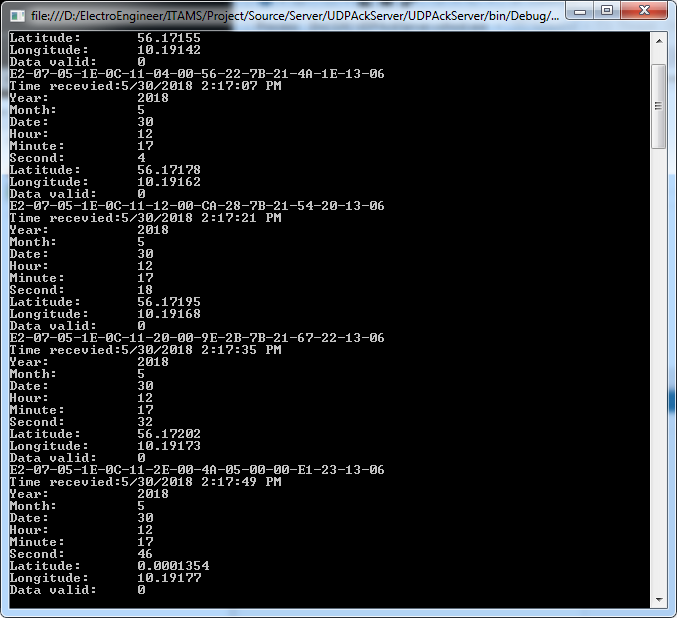
\includegraphics[width=0.9\linewidth]{gfx/Test/AcceptTestConsole.PNG}
	\caption{Server log of acceptance test of \systemName without µSD-card.}
	\label{fig:accepttestconsole}
\end{figure}

\begin{figure}
	\centering
	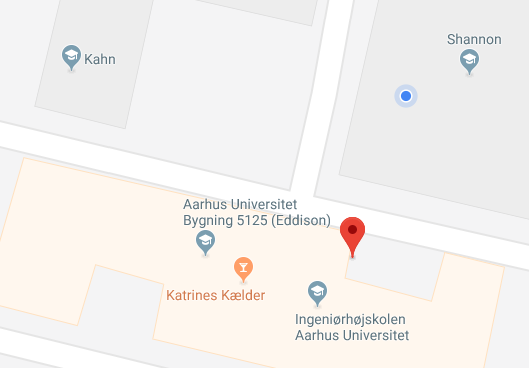
\includegraphics[width=0.7\linewidth]{gfx/Test/AcceptTestMaps.png}
	\caption{Google maps of one of the locations shown in \cref{fig:accepttestconsole}. The blue dot is the actual location, the red is the GPS coordinate. Some of the deviation might be due to the use of float and not double on the server, for storing the coordinates.}
	\label{fig:accepttestmaps}
\end{figure}


\FloatBarrier